%% LyX 2.4.1 created this file.  For more info, see https://www.lyx.org/.
%% Do not edit unless you really know what you are doing.
\documentclass[10pt,english,t]{beamer}
\usepackage{lmodern}
\usepackage[T1]{fontenc}
\usepackage[utf8]{inputenc}
\usepackage{amsbsy}
\usepackage{amstext}
\usepackage{amssymb}
\usepackage{graphicx}
\usepackage[authoryear]{natbib}
\PassOptionsToPackage{normalem}{ulem}
\usepackage{ulem}

\makeatletter

%%%%%%%%%%%%%%%%%%%%%%%%%%%%%% LyX specific LaTeX commands.
%% Because html converters don't know tabularnewline
\providecommand{\tabularnewline}{\\}

%%%%%%%%%%%%%%%%%%%%%%%%%%%%%% Textclass specific LaTeX commands.
% this default might be overridden by plain title style
\newcommand\makebeamertitle{\frame{\maketitle}}%
% (ERT) argument for the TOC
\AtBeginDocument{%
  \let\origtableofcontents=\tableofcontents
  \def\tableofcontents{\@ifnextchar[{\origtableofcontents}{\gobbletableofcontents}}
  \def\gobbletableofcontents#1{\origtableofcontents}
}

%%%%%%%%%%%%%%%%%%%%%%%%%%%%%% User specified LaTeX commands.
\usepackage{tikz}
\usetikzlibrary{positioning}
\usepackage{appendixnumberbeamer}

\usetheme[progressbar=frametitle,block=fill]{metropolis}

% margin
\setbeamersize{text margin right=1.5cm}

% colors
\colorlet{DarkRed}{red!70!black}
\setbeamercolor{normal text}{fg=black}
\setbeamercolor{alerted text}{fg=DarkRed}
\setbeamercolor{progress bar}{fg=DarkRed}
\setbeamercolor{button}{bg=DarkRed}

% width of seperators
\makeatletter
\setlength{\metropolis@titleseparator@linewidth}{1pt}
\setlength{\metropolis@progressonsectionpage@linewidth}{1pt}
\setlength{\metropolis@progressinheadfoot@linewidth}{1pt}
\makeatother

% new alert block
\newlength\origleftmargini
\setlength\origleftmargini\leftmargini
\setbeamertemplate{itemize/enumerate body begin}{\setlength{\leftmargini}{4mm}}
\let\oldalertblock\alertblock
\let\oldendalertblock\endalertblock
\def\alertblock{\begingroup \setbeamertemplate{itemize/enumerate body begin}{\setlength{\leftmargini}{\origleftmargini}} \oldalertblock}
\def\endalertblock{\oldendalertblock \endgroup}
\setbeamertemplate{mini frame}{}
\setbeamertemplate{mini frame in current section}{}
\setbeamertemplate{mini frame in current subsection}{}
\setbeamercolor{section in head/foot}{fg=normal text.bg, bg=structure.fg}
\setbeamercolor{subsection in head/foot}{fg=normal text.bg, bg=structure.fg}

% footer
\makeatletter
\setlength{\metropolis@frametitle@padding}{1.6ex}
\setbeamertemplate{footline}{%
    \begin{beamercolorbox}[colsep=1.5pt]{upper separation line head}
    \end{beamercolorbox}
    \begin{beamercolorbox}{section in head/foot}
      \vskip1pt\insertsectionnavigationhorizontal{\paperwidth}{}{\hskip0pt plus1filll \insertframenumber{} / \inserttotalframenumber \hskip2pt}\vskip3pt% 
    \end{beamercolorbox}%
    \begin{beamercolorbox}[colsep=1.5pt]{lower separation line head}
    \end{beamercolorbox}
}
\makeatother

% toc
\setbeamertemplate{section in toc}{\hspace*{1em}\inserttocsectionnumber.~\inserttocsection\par}
\setbeamertemplate{subsection in toc}{\hspace*{2em}\inserttocsectionnumber.\inserttocsubsectionnumber.~\inserttocsubsection\par}
% Added by lyx2lyx
\setlength{\parskip}{\smallskipamount}
\setlength{\parindent}{0pt}

\makeatother

\usepackage{babel}
\begin{document}
\title{Macroeconomics II: Course Summary \vspace{-4mm}}
\author{\vspace{-4mm}\footnotesize
Erik Öberg (Uppsala University, UCLS)\vspace{4mm}
}

{
\date{May 15, 2023}
\setbeamertemplate{footline}{} 
\begin{frame}

\maketitle

\end{frame}
}

\addtocounter{framenumber}{-1}
\begin{frame}{What have we covered?}
\begin{itemize}
\item \textbf{Business-cycle frameworks:} \emph{RBC, NK}
\item \textbf{Fricitional labor markets: }McCall, Burdett-Mortensen, DMP
\item \textbf{Incomplete asset markets: }Consumption-savings dynamics in
partial equilibrium, Aiyagari
\end{itemize}
\end{frame}
%
\begin{frame}{Today}
\begin{itemize}
\item Apart from the RBC extensions, we have focused on the ``vanilla''
versions of these frameworks in isolation
\item Today: attempt to summarize the course material, by means of showing
how these frameworks can be put together and are used for quantitative
research
\item In particular, we will outline a business cycle model with sticky
prices, incomplete asset markets and a frictional labor market: a
\textbf{HANK-SAM Model}
\end{itemize}
\end{frame}
%
\begin{frame}{HANK models}
\begin{itemize}
\item \textbf{Heterogeneous Agents New Keynesian} models: NK business cycle
models with incomplete asset markets (and therefore household heterogeneity)
\item Why interesting?
\item Consider the vanilla RANK model:
\begin{eqnarray*}
\hat{i}_{t} & = & \phi\pi_{t}+\nu_{t}\\
\pi_{t} & = & \beta E_{t}\pi_{t+1}+\kappa\hat{y}_{t}\\
\hat{y}_{t} & = & -(\hat{i}_{t}-E_{t}\pi_{t+1})+E_{t}\hat{y}_{t+1}
\end{eqnarray*}
\item What is the transmission mechanism of an MP shock?
\end{itemize}
\end{frame}
%
\begin{frame}{HANK models}
\begin{itemize}
\item Extended representation of the vanilla RANK model:
\begin{eqnarray*}
\hat{i}_{t} & = & \phi\pi_{t}+\nu_{t}\\
\pi_{t} & = & \beta E_{t}\pi_{t+1}+\kappa\hat{y}_{t}\\
\hat{c}_{t} & = & -(\hat{i}_{t}-E_{t}\pi_{t+1})+E_{t}\hat{c}_{t+1}\\
\hat{c_{t}} & = & \hat{y_{t}}
\end{eqnarray*}
\item What is the transmission mechanism of an MP shock to output? Roughly:
\begin{enumerate}
\item Shock: nominal rate $i_{t}$ up
\item Sticky prices: real rate $\hat{i}_{t}-E_{t}\pi_{t+1}$ up
\item Intertemporal substitution: consumption $c_{t}$ down
\item Market clearing: output $y_{t}$ down
\end{enumerate}
\end{itemize}
\end{frame}
%
\begin{frame}{HANK models: motivation}
\begin{itemize}
\item Is intertemporal substitution really a reasonable theory of fluctuations
in aggregate demand?
\begin{itemize}
\item Macro evidence: no (see, e.g., Yogo, ReStat 2004; Canzoneri-Cumby-Dilba,
JME 2007)
\item Micro evidence: Limited, but also no (see, e.g., Best-Cloyne-Ilzetski-Kleven,
REStud 2020)
\end{itemize}
\item Even though income, financial wealth and income risk might respond
to monetary policy as well, this has close to no impact on the consumption
decisions of well-insured households
\begin{itemize}
\item Recall lecture 10: well-insured households behaves according to PIH
\end{itemize}
\item This is counterintuitive and at odds with what we know from the micro
data
\item HANK models offer an alternative theory of aggregate demand
\end{itemize}
\end{frame}
%
\begin{frame}{HANK models: new transsmission mechanisms}

{\centering%
\begin{tabular}{c}
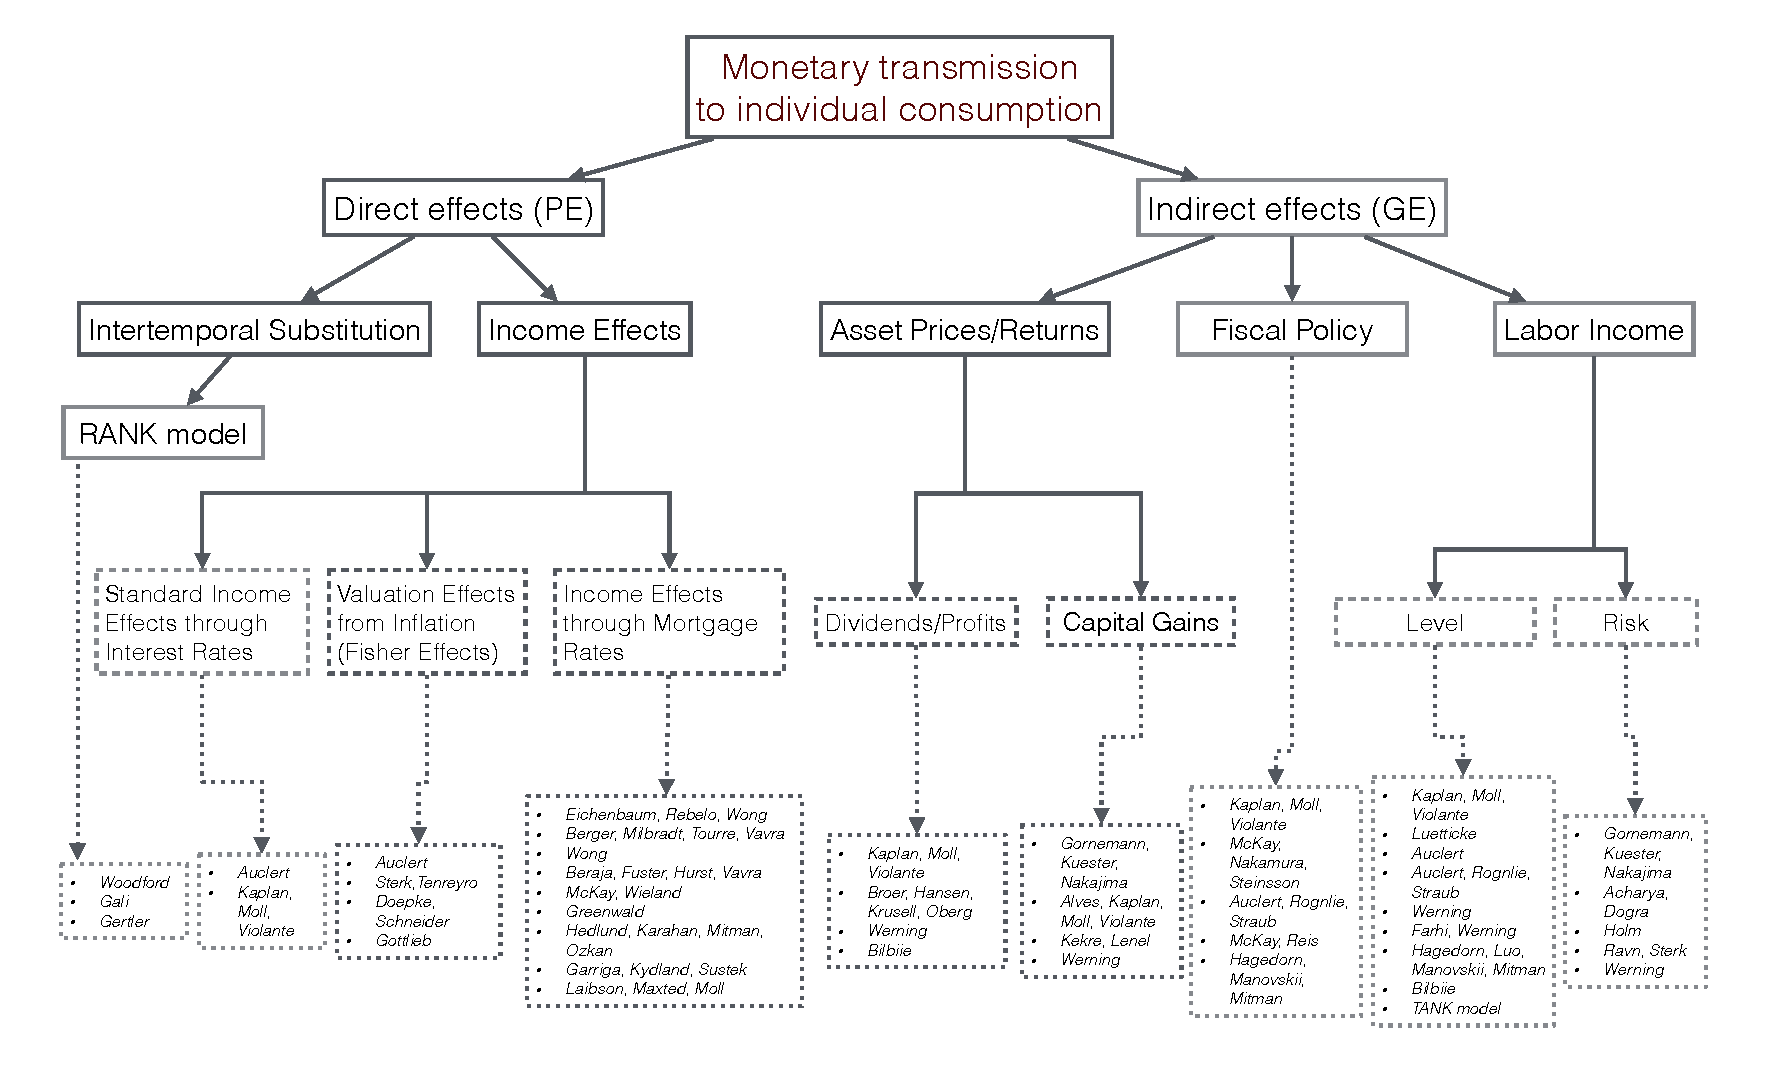
\includegraphics[width=1\textwidth]{figs/HANK_summary}\tabularnewline
\end{tabular}

}Taken from Ben Moll's website
\end{frame}
%
\begin{frame}{The Unemployment Risk Channel}
\begin{itemize}
\item One channel that has attracted much attention: \textbf{Unemployment-risk
channel (URC)}
\begin{enumerate}
\item \textbf{Households:} Unemployment $\uparrow$ \\
$\Rightarrow$ precautionary saving $\uparrow$ \\
$\Rightarrow$ goods demand $\downarrow$
\item \textbf{Firms:} Goods demand $\downarrow$ \\
$\Rightarrow$ labor demand $\downarrow$ \\
$\Rightarrow$ unemployment $\uparrow$
\end{enumerate}
\item Generates a multiplier
\begin{enumerate}
\item \emph{Inefficient }amplification \& propagation
\item May be mitigated with targeted fiscal policy
\end{enumerate}
\item To evaluate the implications of this channel, we need a HANK model
with endogenous unemployment dynamics: \textbf{HANK-SAM models}
\end{itemize}
\end{frame}
%
\begin{frame}{HANK-SAM models}
\begin{itemize}
\item \textbf{Ravn-Sterk (JME 2017; JEEA 2021), Rendahl-Riegler-Den Haan
(JEEA 2019): }HANK-SAM interaction is a source of amplification
\item \textbf{McKay-Reis (Ecmtra 2016; REStud 2021), Kekre (REStud forthc):
}HANK-SAM interaction raises the value of automatic stabilizers (esp
unempl. insurance)
\item \textbf{Challe (AEJmacro 2020):} HANK-SAM interaction changes optimal
monetary policy
\item \textbf{Broer-Druedahl-Harmenberg-Öberg (no paper yet): }A unified
framework to evaluate the cost-effectiveness of different fiscal stabilization
policies
\item To illustrate some of these points, I will employ a (slightly simplified)
version of the framework in BDHÖ
\end{itemize}
\end{frame}
%
\begin{frame}{A HANK-SAM Model}
\begin{itemize}
\item \vspace{-2mm}\textbf{Households:}
\begin{enumerate}
\item \textbf{Workers: }can be \emph{employed }or \emph{unemployed}
\begin{itemize}
\item Employed: Earn fixed real wage $W$, pay labor income taxes
\item Unemployed: enjoy UI benefits
\end{itemize}
\item \textbf{Capitalists: }collect all firm profits, do not work, risk
neutral
\end{enumerate}
\item \textbf{Producers:}
\begin{enumerate}
\item \textbf{Intermediate good producers}
\begin{itemize}
\item Labor $\Rightarrow$intermediate goods
\item Frictional labor market, CRS matching function
\item Sluggish vacancy posting due to \uline{idiosyncratic stochastic entry
cost}
\item Separations due to \uline{idiosyncratic stochastic continuation cost}
\end{itemize}
\item \textbf{Wholesale producers}
\begin{itemize}
\item Intermediate goods $\Rightarrow$ differentiated goods
\item Monopolistic competition + Rotemberg price adjustment costs
\end{itemize}
\item \textbf{Final producers}
\begin{itemize}
\item Differentiated goods $\Rightarrow$ final good
\item Perfect competition
\end{itemize}
\end{enumerate}
\item \textbf{Government:} Sets the nominal interest rate, collects taxes,
issues debt
\end{itemize}
\end{frame}
%
\begin{frame}{Graphical model overview}

\vspace{-2mm}\includegraphics[bb=0bp 0bp 656bp 190bp,clip,width=1.1\linewidth]{../../../../../../research/persistent_income_risk/presentations/Amsterdam_may2023/figs/model_diagram}\vspace{-5mm}
\begin{itemize}
\item Consider an exogenous path of TFP $\boldsymbol{\boldsymbol{z}}\boldsymbol{=}[z_{0},z_{1},...]$
\item To a first-order approximation, the equilibrium is summarized by\vspace{1mm}
\begin{enumerate}
\item <+->\textbf{A SAM-block response}: $\boldsymbol{u}\boldsymbol{=}M_{SAM}(\boldsymbol{p^{x}+}\boldsymbol{z})$

$\mathbf{u}$ is the path of unemployment \emph{and} the labor-market
flows\vspace{1mm}
\item <+->\textbf{An HA-block response}: \textbf{$\boldsymbol{\boldsymbol{R}^{real}=}M_{HA}\boldsymbol{u}$}\vspace{1mm}
\item <+->\textbf{An NK-block response}: \textbf{$\boldsymbol{p^{x}}\boldsymbol{=}M_{NK}\boldsymbol{R^{real}}$}\vspace{1mm}
\end{enumerate}
\end{itemize}
\end{frame}
%
\begin{frame}{The multiplier process}

\vspace{-2mm}\includegraphics[bb=0bp 0bp 656bp 190bp,clip,width=1.1\linewidth]{../../../../../../research/persistent_income_risk/presentations/Amsterdam_may2023/figs/model_diagram}\vspace{-5mm}
\begin{itemize}
\item \textbf{Proposition: }Model solution is given by
\[
\boldsymbol{u}=(I-M_{\text{SAM}}M_{\text{NK}}M_{\text{HA}})^{-1}M_{SAM}\mathbf{z}
\]

\begin{enumerate}
\item $(I-M_{\text{SAM}}M_{\text{NK}}M_{\text{HA}})^{-1}$ captures a repeated
\textbf{demand-driven }multiplier process generating the equilibrium
response to the shock
\item The direct (first-round) response $\boldsymbol{u}=M_{SAM}\mathbf{z}$
is also the response with \emph{flexible prices} (no demand-loop)
\end{enumerate}
\end{itemize}
\end{frame}
%
\begin{frame}{The multiplier process: illustration}

\begin{tabular}{cc}
TFP, $Z_{t}$ & Unemployment Risk, $URISK_{t}$\tabularnewline
{\small\textbf{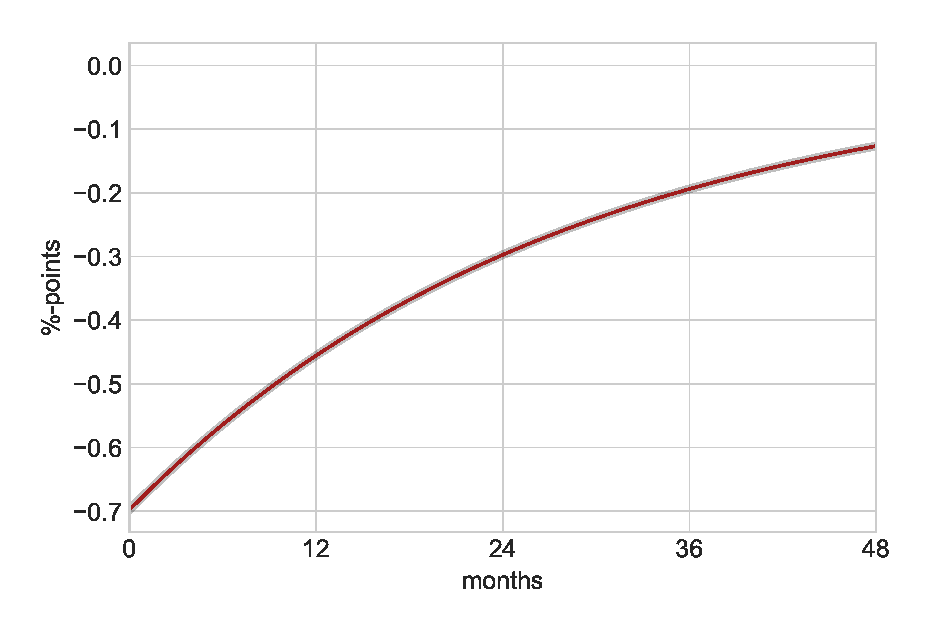
\includegraphics[width=0.45\textwidth]{results/TFP_multiplier_TFP}}} & {\small\textbf{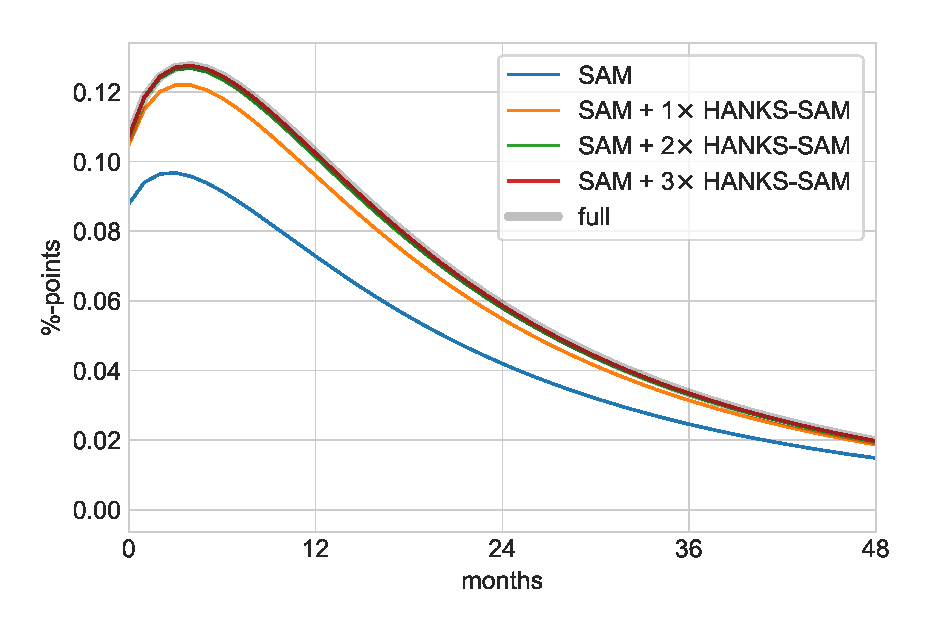
\includegraphics[width=0.45\textwidth]{results/TFP_multiplier_urisk}}}\tabularnewline
Intermediate goods price, $P_{t}^{x}$ & Unemployment, $U_{t}$\tabularnewline
{\small\textbf{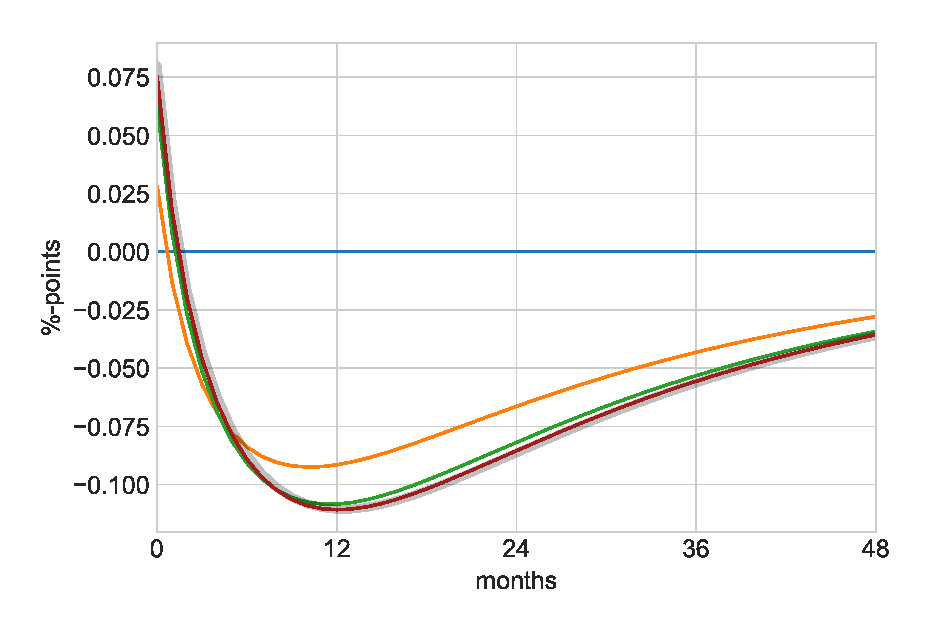
\includegraphics[width=0.45\textwidth]{results/TFP_multiplier_px}}} & {\small\textbf{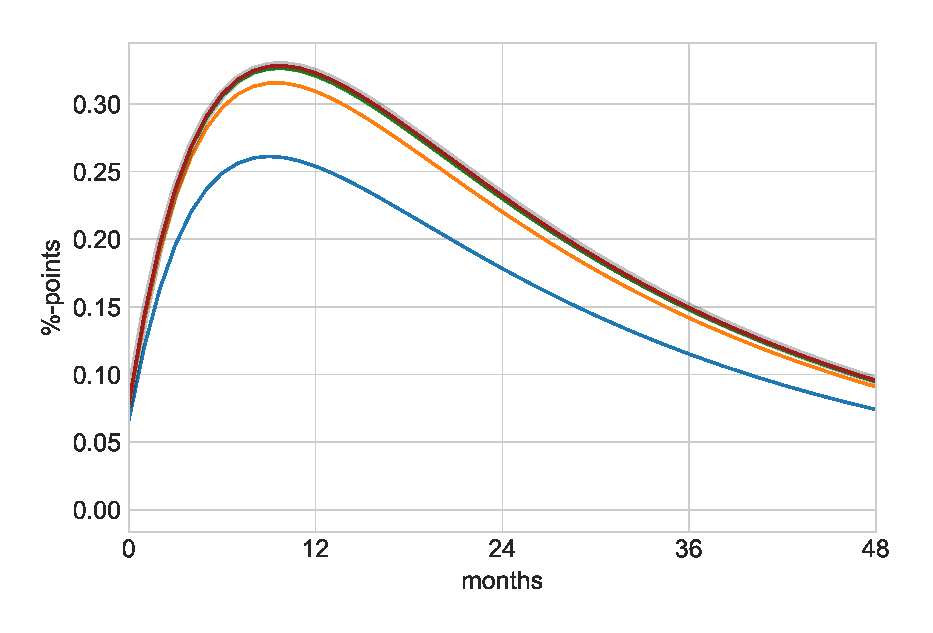
\includegraphics[width=0.45\textwidth]{results/TFP_multiplier_u}}}\tabularnewline
\end{tabular}
\end{frame}
%
\begin{frame}{Equivalence of demand and supply shocks}
\begin{itemize}
\item \textbf{Proposition: }The impulse responses for labor-market variables
to a shock to TFP (supply) and to the discount factor of workers (demand)
are equivalent up to a scaling factor.
\item Interesting, because IRFs of labor market variables to TFP and MP
shocks look very similar in the data (at odds with vanilla NK model!)
\end{itemize}
\end{frame}
%
\begin{frame}{Equivalence of shocks in the model: illustration}
\begin{center}
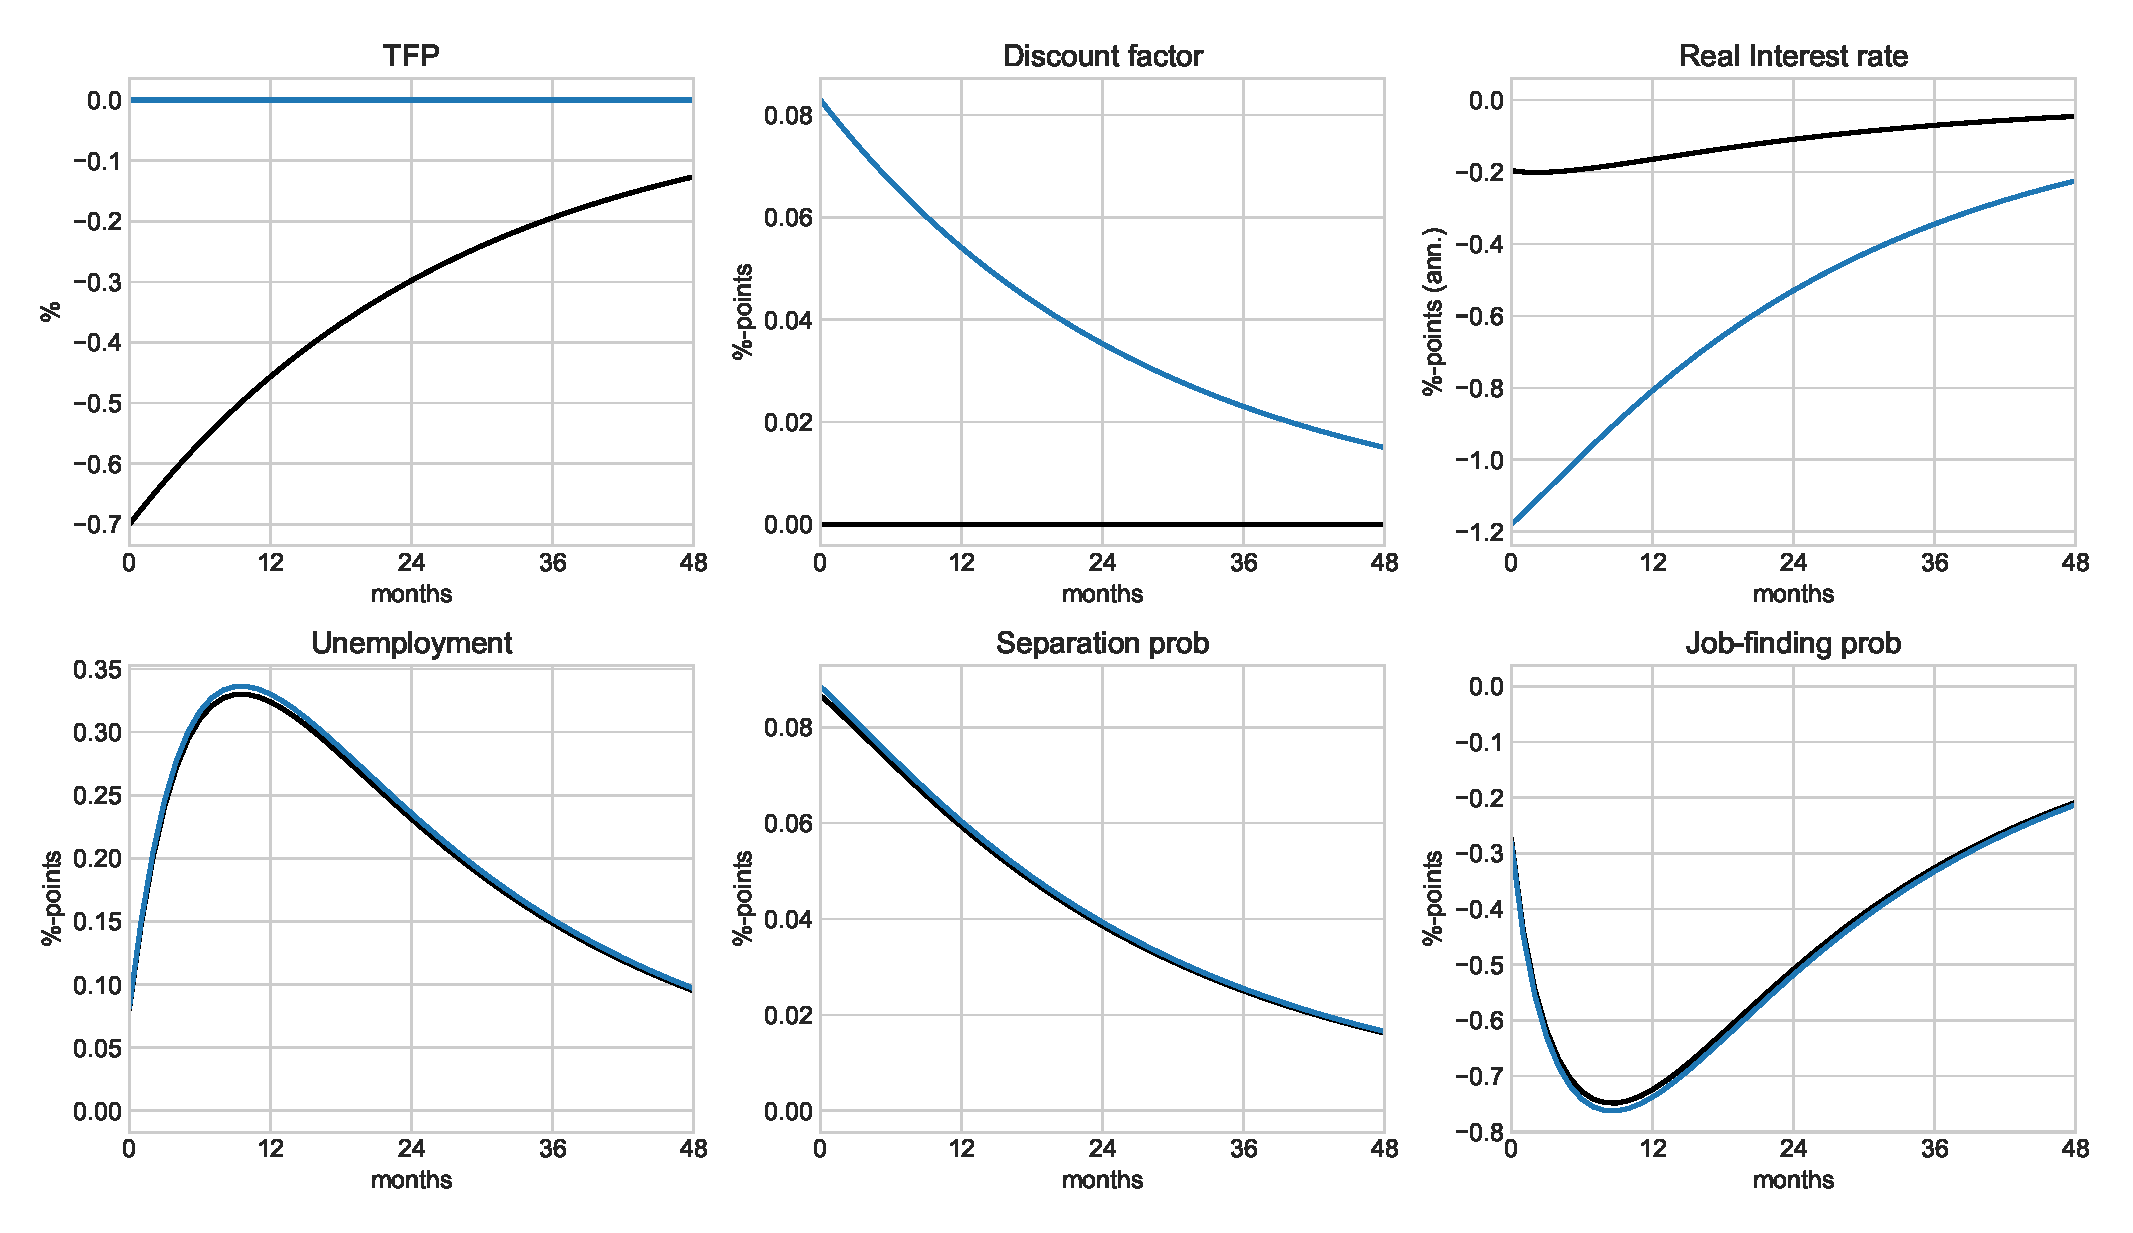
\includegraphics[width=0.95\textwidth]{figs/demand_supply_irf_set}
\par\end{center}

\end{frame}
%
\begin{frame}{Our calibration approach}
\begin{itemize}
\item \textbf{Calibrate HA block} so consumption-saving of households match
evidence on
\begin{enumerate}
\item Fall in consumption in response to unemployment
\item Fall in consumption in response to unemployment-benefit expiration
\item Marginal propensity to consume (not targeted but in line with data)
\end{enumerate}
\item \textbf{Calibrate SAM block} so firing-hiring of firms match evidence
on
\begin{enumerate}
\item Relative timing of the peak for the separation rate and \\
the trough for the job-finding rate
\item Contribution of separation and the job-finding rate to unemployment
dynamics
\end{enumerate}
\end{itemize}
\end{frame}
%
\begin{frame}{Consumption effects of unemployment}

\begin{itemize}
\item \textbf{Stylized fact \#1: }Consumption \textasciitilde 20\% lower
for unemployed (Chodorow-Reich-Karabarbounis, 2016)
\item \textbf{Stylized fact \#2: }Drop at UI exhaustion of \textasciitilde 45\%
of income drop (Ganong-Noel, 2019)
\end{itemize}
\begin{center}
\includegraphics[width=0.7\linewidth]{../../../../../../research/persistent_income_risk/presentations/Amsterdam_may2023/figs/Ganong19}
\par\end{center}

\begin{center}
\vspace{-3mm}{\footnotesize\textbf{Source:}}{\footnotesize{} Ganong-Noel
(2019)}{\footnotesize\par}
\par\end{center}

\end{frame}
%
\begin{frame}{\emph{Separation rate leads job-finding rate}}

\begin{tabular}{cc}
\textbf{Monetary policy shock} & \textbf{Technology shock}\tabularnewline
{\small\textbf{\includegraphics[width=0.5\textwidth]{../../../../../../research/persistent_income_risk/presentations/Amsterdam_may2023/results/monetary_shock_lead_lag}}} & {\small\textbf{\includegraphics[width=0.5\textwidth]{../../../../../../research/persistent_income_risk/presentations/Amsterdam_may2023/results/technology_shock_lead_lag}}}\tabularnewline
\end{tabular}

{\footnotesize\textbf{Source: }}{\footnotesize CPS 1967-2020; Romer-Romer
MP shock; Fernald TFP shock}.\vspace{3mm}

\begin{itemize}
\item \textbf{Stylized Fact \#3:}\emph{}\\
\emph{Separation rate leads job-finding rate by 9-16 months}\vspace{3mm}
\item Also true for \emph{uncertainty shocks} (Oh-Picco, 2020)
\end{itemize}
\end{frame}
%
\begin{frame}{\emph{Separation rate explains substantial share of unemployment}}

\begin{tabular}{cc}
\textbf{Monetary policy shock} & \textbf{TFP shock}\tabularnewline
{\small\textbf{\includegraphics[width=0.5\textwidth]{../../../../../../research/persistent_income_risk/presentations/Amsterdam_may2023/results/monetary_shock_decomposition}}} & {\small\textbf{\includegraphics[width=0.5\textwidth]{../../../../../../research/persistent_income_risk/presentations/Amsterdam_may2023/results/technology_shock_decomposition}}}\tabularnewline
\end{tabular}

{\footnotesize\textbf{Source: }}{\footnotesize CPS 1967-2020; Romer-Romer
MP shock; Fernald TFP shock}.\vspace{3mm}
\begin{itemize}
\item \textbf{Stylized Fact \#4:}\emph{}\\
\emph{Separations account for 40-60 percent of unemployment response}\vspace{3mm}
\item Also true for \emph{uncertainty shocks} (Oh-Picco, 2020)
\end{itemize}
\end{frame}
%
\begin{frame}{To explain separation rate response, our model has elastic job destruction}
\begin{itemize}
\item \textbf{Job value:} 
\begin{eqnarray*}
V_{t}^{j} & = & P_{t}^{x}Z_{t}-W+\beta\mathbb{E}_{t}\left[(1-\delta_{t+1})(V_{t+1}^{j}-\mu_{t+1})\right]
\end{eqnarray*}

\begin{itemize}
\item TFP: $Z_{t}$
\item Real output price: $P_{t}^{x}$
\item Wage: $W$
\item Separation rate: $\delta_{t}$
\item Continuation cost: $\mu_{t}$
\end{itemize}
\item \textbf{Firms draw continuation cost} $\chi_{t}\sim G$: mixture of
point-mass and Pareto
\item \textbf{Implied separation rate: 
\[
\delta_{t}=\delta_{ss}\left(\frac{V_{t}^{j}}{V_{ss}^{j}}\right)^{-\psi}
\]
}
\item \textbf{Exogenous separation limit:} $\psi\rightarrow0$
\end{itemize}
\end{frame}
%
\begin{frame}{To explain job-finding rate response, our model has inelastic job
creation}
\begin{itemize}
\item \textbf{Vacancy value:} 
\begin{eqnarray*}
V_{t}^{v} & = & -\kappa+\lambda_{t}^{v}V_{t}^{j}+(1-\lambda_{t}^{v})\beta\mathbb{E}_{t}\left[V_{t+1}^{v}\right]
\end{eqnarray*}

\begin{itemize}
\item Vacancy posting cost: $\kappa$
\item Job-filling rate: $\lambda_{t}^{v}$
\end{itemize}
\item \textbf{Firms draw entry cost $c\sim H$: }exponential distribution\textbf{ }
\item \textbf{Implied entry
\[
\iota_{t}=\iota_{ss}\left(\frac{V_{t}^{v}}{V_{ss}^{v}}\right)^{\frac{1}{\xi}}
\]
}
\item \textbf{Free entry model: }$\xi\rightarrow\infty$, $V_{ss}^{v}\rightarrow0$

(Only $\xi\rightarrow\infty$: Fixed homogenous entry cost)
\end{itemize}
\end{frame}
%
\begin{frame}{Demand externality matters only with active URC}

\begin{tabular}{cl}
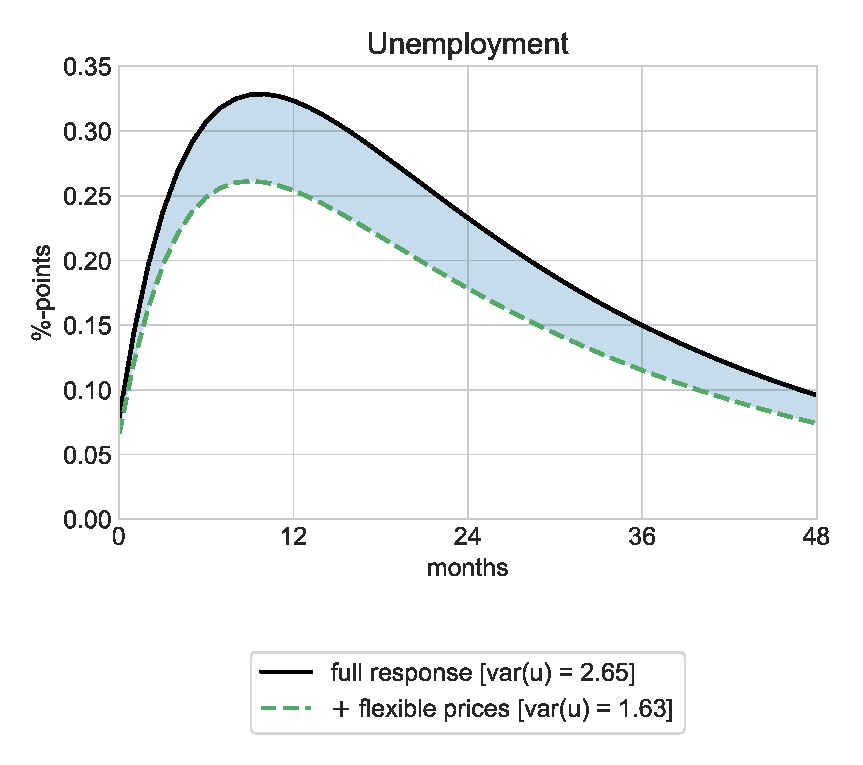
\includegraphics[width=0.5\linewidth]{results/decompositionmultiplier} & 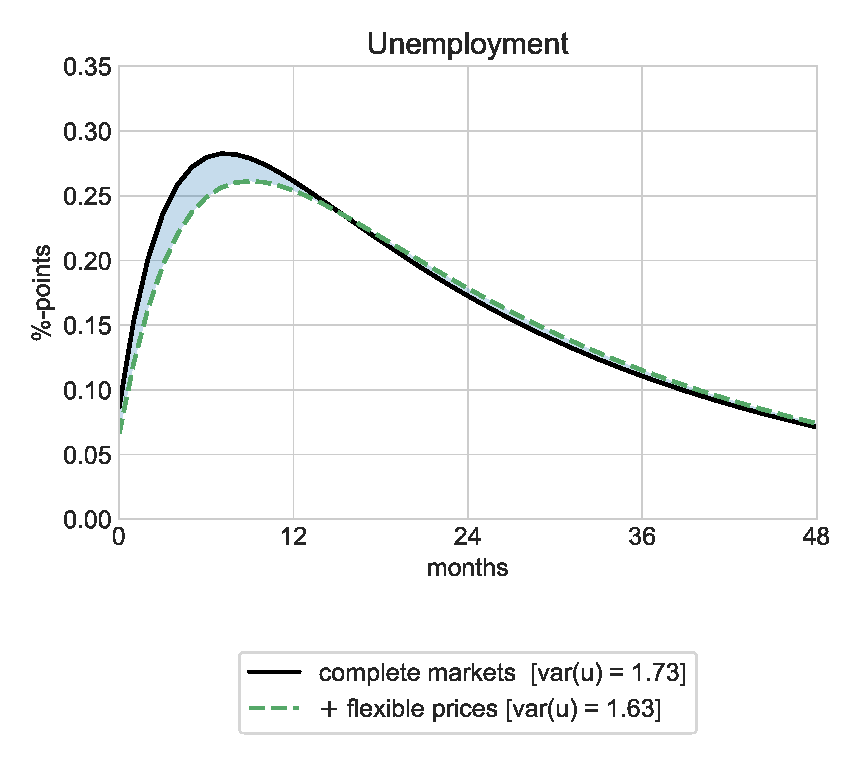
\includegraphics[width=0.5\linewidth]{results/decompositionmultiplier_complete}\tabularnewline
\end{tabular}
\begin{itemize}
\item \textbf{Baseline with incomplete markets:} substantial amplification
with sticky prices
\item \textbf{With complete markets}: only aggregate income path matters;
sticky prices make little difference
\end{itemize}
\end{frame}
%
\begin{frame}{Substantial amplification due to elastic firing and inelastic hiring}

\begin{tabular}{cc}
\textbf{Unemployment} & \textbf{Unemployment gap (com. mkts)}\tabularnewline
{\small\textbf{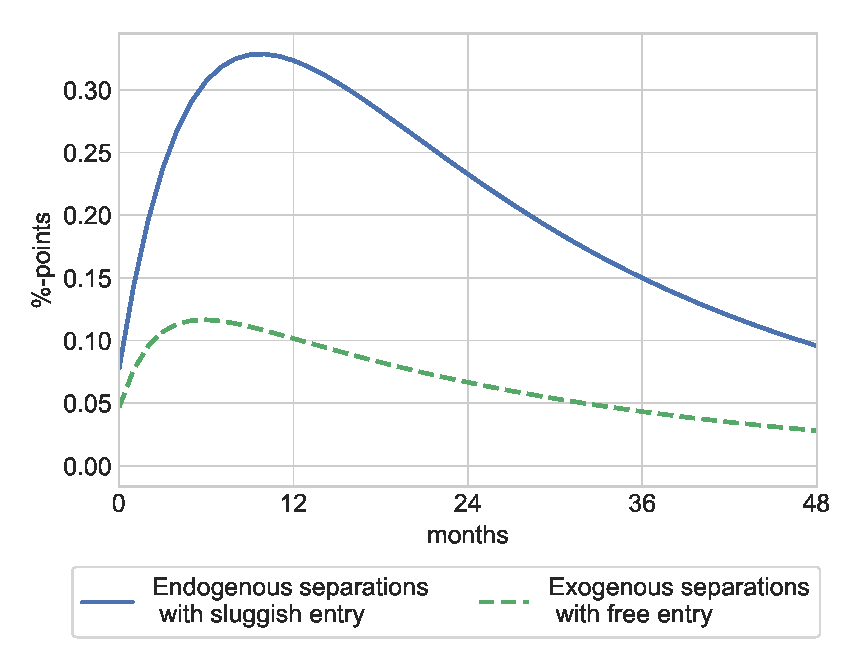
\includegraphics[width=0.5\textwidth]{results/interaction_simple}}} & {\small\textbf{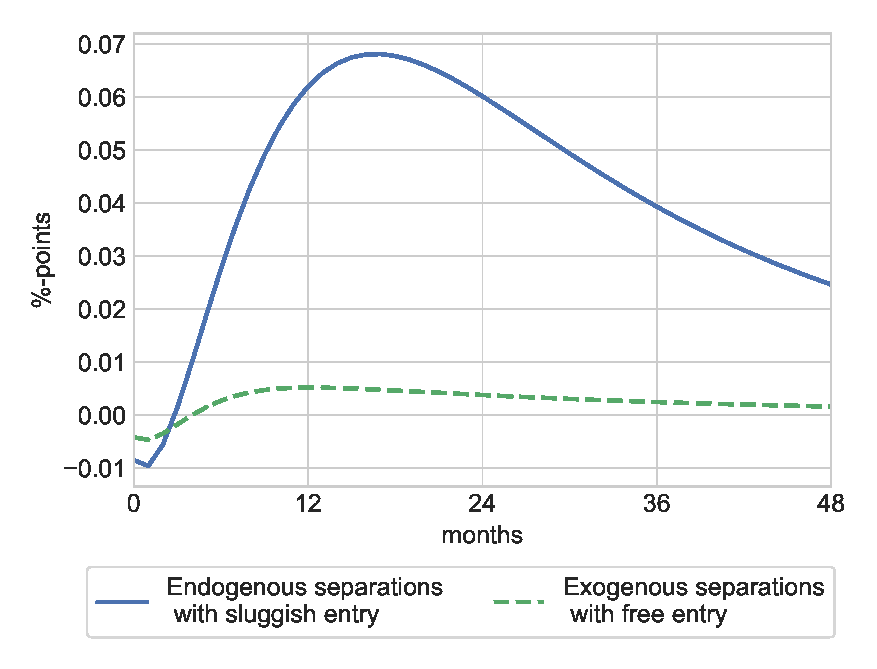
\includegraphics[width=0.5\textwidth]{results/interaction_gap_simple}}}\tabularnewline
\end{tabular}
\begin{itemize}
\item \vspace{-5mm}\textbf{Standard HANK-SAM} (exo. sep., free entry):
\begin{enumerate}
\item Much smaller unemployment response
\end{enumerate}
\end{itemize}
\end{frame}
%
\begin{frame}{Interaction of elastic firing and inelastic hiring}

\begin{tabular}{cc}
\textbf{Unemployment} & \textbf{Unemployment gap (com. mkts)}\tabularnewline
{\small\textbf{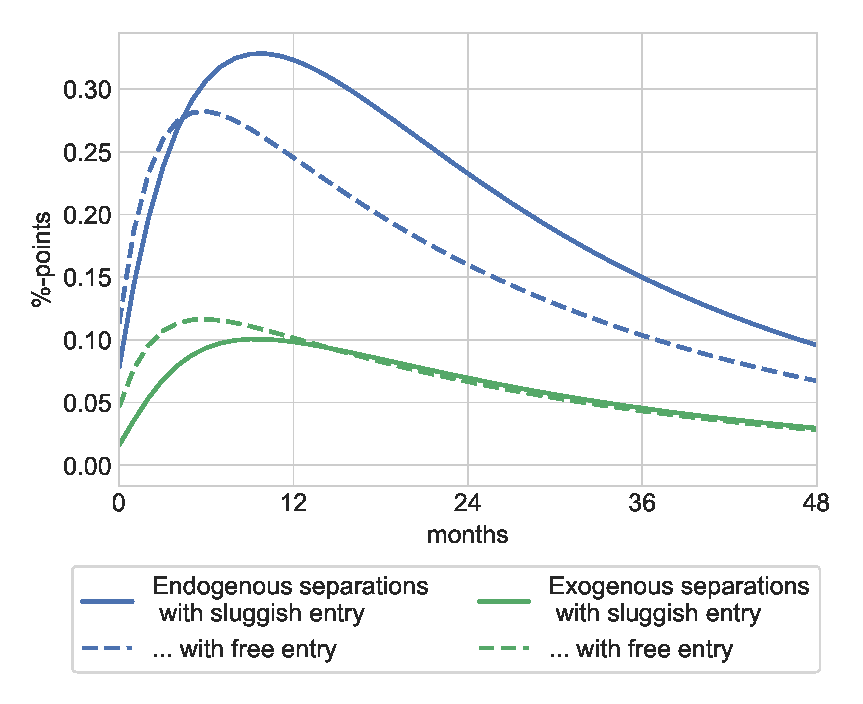
\includegraphics[width=0.5\textwidth]{results/interaction}}} & {\small\textbf{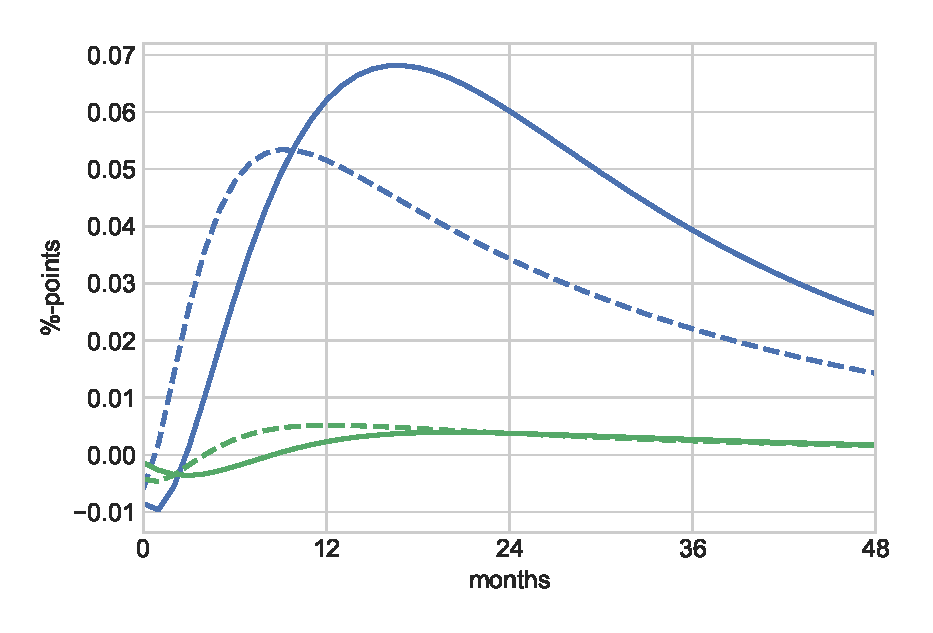
\includegraphics[width=0.5\textwidth]{results/interaction_gap}}}\tabularnewline
\end{tabular}
\begin{enumerate}
\item \vspace{-5mm}\textbf{Endogenous separations} always amplifies
\item \textbf{Sluggish entry} \emph{only amplifies with endogenous separations}
\begin{itemize}
\item With limited entry response, newly separated \emph{deplete the current
vacancy stock}
\item $\Rightarrow$Higher separation rate causes lower job-finding rate 
\end{itemize}
\end{enumerate}
\end{frame}
%
\begin{frame}{Back to the litterature}
\begin{itemize}
\item \textbf{Ravn-Sterk (JME 2017; JEEA 2021), Rendahl-Riegler-Den Haan
(JEEA 2019): }HANK-SAM interaction is a source of amplification
\begin{itemize}
\item These models typically features a large demand-driven multiplier
\end{itemize}
\item \textbf{McKay-Reis (Ecmtra 2016; REStud 2021), Kekre (REStud forthc):
}HANK-SAM interaction raises the value of automatic stabilizers (esp
unempl. insurance)
\begin{itemize}
\item The demand-driven multiplier stems from limited insurance to unemployment
risk
\end{itemize}
\item \textbf{Challe (AEJmacro 2020):} HANK-SAM interaction changes optimal
monetary policy
\begin{itemize}
\item The demand-driven multiplier changes the trade-off between stabilizing
inflation and output
\end{itemize}
\end{itemize}
\end{frame}
%
\begin{frame}{Back to the litterature}
\begin{itemize}
\item \textbf{Broer-Druedahl-Harmenberg-Öberg (no paper yet): }A unified
framework to evaluate the cost-effectiveness of different fiscal stabilization
policies
\begin{itemize}
\item Commonly used labor-market policies (e.g. retention policies, hiring
subsidies) may be very effective macroeconomic stabilization tools
\item Whether labor-market policies are preferable over UI (and other fiscal
polciies) depend very much on the elasticity of job creation and job
destruction
\item We need more micro-level evidence on these elasticities
\end{itemize}
\end{itemize}
\end{frame}
%

\end{document}
